\begin{enumerate}[label=\thesection.\arabic*.,ref=\thesection.\theenumi]
\numberwithin{equation}{enumi}
\numberwithin{figure}{enumi}
%%
\item Let 
\begin{equation}
\mbf{y} = A\mbf{x} + \mbf{n},
\end{equation}
where 
\begin{align}
x &\in \brak{\mbf{s}_0,\mbf{s}_1}, 
\mbf{s}_0 = 
\begin{pmatrix}
1 
\\
0
\end{pmatrix},
\mbf{s}_1 = 
\begin{pmatrix}
0 
\\
1
\end{pmatrix}
\\
\mbf{n} &= 
\begin{pmatrix}
n_1
\\
n_2
\end{pmatrix},
n_1,n_2 \sim \gauss{0}{1}.
\end{align}
%
\item
\label{ch5_fsk}
Plot 
%
\begin{equation}
\mbf{y}|\mbf{s}_0 \text{ and } \mbf{y}|\mbf{s}_1
\end{equation}
%
on the same graph using a scatter plot.
\\
\clearpage
\solution The following python code plots the scatter plot when $\mbf{x} = \mbf{s}_0$ and $\mbf{x} = \mbf{s}_1$ in Fig. \ref{fig:scatter_plt_y}
\begin{lstlisting}
codes/twoD/scatter_plot.py
\end{lstlisting}
\begin{figure}
\centering
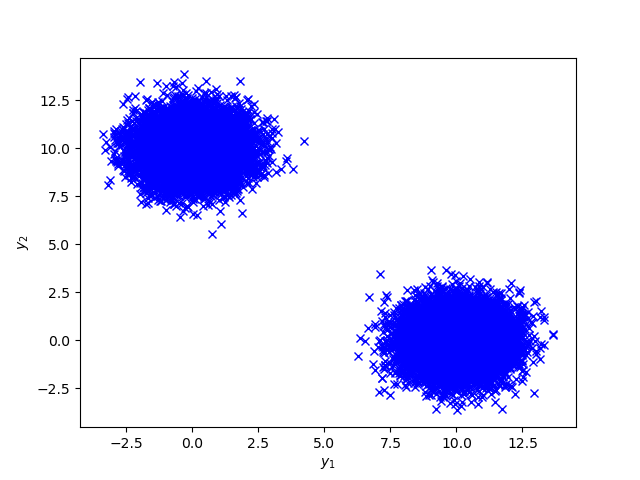
\includegraphics[width=\columnwidth]{./figs/twoD/scatter_plot.png}
\caption{Scatter plot of $\mbf{y} = \begin{pmatrix} y_1 \\ y_2 \end{pmatrix}$ for $A = 10$}
\label{fig:scatter_plt_y}
\end{figure}
%
\item
For the above problem, find a decision rule for detecting the symbols $\mbf{s}_0 $ and $\mbf{s}_1$.
\\
\solution The decision rule is
\begin{equation}
\label{eq:decision_rule}
y_1 \dec{s_0}{s_1} y_2
\end{equation}
%
\item
Plot 
\begin{equation} 
P_e = \pr{\hat{\mbf{x}} = \mbf{s}_1|\mbf{x} = \mbf{s}_0}
\end{equation}
with respect to the SNR from 0 to 10 dB.
\\
\begin{figure}
\centering
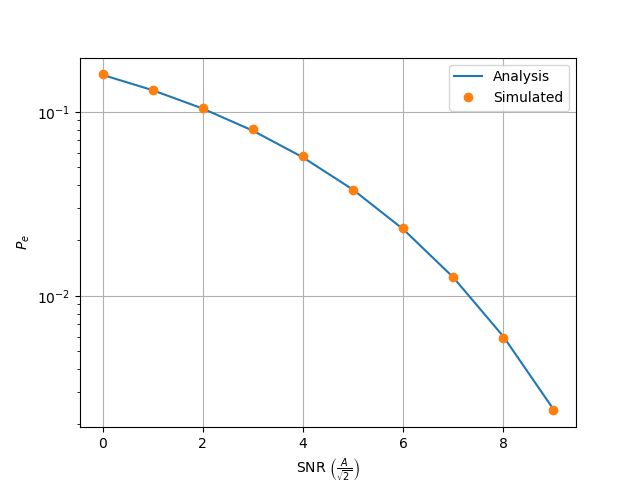
\includegraphics[width=\columnwidth]{./figs/twoD/ber_snr_plot.png}
\caption{$P_e$ with respect to SNR from 0 to 10 dB}
\label{fig:ber_snr_plot}
\end{figure}
%
\item
Obtain an expression for $P_e$. Verify this by comparing the theory and simulation plots on the same graph.
\\
\solution 
\begin{align}
P_e = \pr{\hat{\mbf{x}} = \mbf{s}_1|\mbf{x} = \mbf{s}_0}
\end{align}
Given that $\mbf{s}_0$ was transmitted, the received signal is
\begin{align}
\mbf{y}|\mbf{s}_0 = \begin{pmatrix} A \\ 0 \end{pmatrix} + \begin{pmatrix} n_1 \\ n_2 \end{pmatrix}
\end{align}
From (\ref{eq:decision_rule}), the probability of error is given by 
\begin{align}
P_e &= \pr{y_1 < y_2 |\mbf{s}_0} = \pr{A+n_1 < n_2}\\
&= \pr{n_2 - n_1 > A}
\end{align}
Note that $n_2 - n_1 \sim \gauss{0}{2}$. Thus,
\begin{align}
P_e &= \pr{\sqrt{2}w > A}\\
\pr{w > \dfrac{A}{\sqrt{2}}}\\
\Rightarrow P_e &= \qfunc{\frac{A}{\sqrt{2}}}
\end{align}
where $w \sim \gauss{0}{1}$. The following code plots the $P_e$ curve in Fig. \ref{fig:ber_snr_plot}.
\begin{lstlisting}
codes/twoD/ber_snr_plot.py
\end{lstlisting}
\end{enumerate}
